% chap2.tex


\chapter{Direct Volume rendering using raycasting}\label{chap:errors}


A 3D dataset normally consists of around one hundred slices, but in some cases, it can be many hundreds of slices. In medical usage, it is a normal practice for radiologists, or medical practitioners to visually inspect each slice~\cite{62}. The common landmarks, such as the major blood vessels or skeleton will be identified, and the locations of the abnormalities will be determined based on these landmarks. Then, they need to mentally visualize the anatomy of the patient with the associated abnormalities,  a task that needs a lot of experience and knowledge. Thus, the process of identifying the structures based on the 2D slices is very tedious, time consuming, and prone to error and could impact the decision on treatment planning. Therefore, volume rendering techniques are needed in order to fully utilize the information of 3D datasets.

The term volume rendering is used to describe techniques which allow the visualization of three-dimensional data. It is a technique for visualizing sampled functions of three spatial dimensions by computing 2-D projections of a colored semi-transparent volume, as shown in figure 2.6. In scientific visualization and computer graphics, volume rendering is a set of techniques used to display a 2D projection of a 3D discretely sampled data set, typically a 3D scalar field. 3D datasets can be structured, unstructured or hybrid grids. 


\section{Introduction}

Classification is a term that refers to assignment of optical properties to data values. Classification is one the most important steps in the volume rendering pipeline, since it is these optical properties that will either emphasize an feature or de-emphasize it. The assignment of optical properties to data values is accomplished using a transfer function. Some applications of classification are:

\begin{itemize}

\item Isosurfaces can be shown by mapping boundary elements of corresponding data values to almost opaque values and the rest to transparent values. The appearance of surfaces can be improved by using shading techniques to form the RGB mapping. 

\item Opacity can be used to see the interior of the data volume too. These interiors appear as clouds with varying density and color. A big advantage of volume rendering is that this interior information is not thrown away, so that it enables one to look at the 3D data set as a whole. 

\end{itemize}

\section{Definitions}

\subsection{3D Grid}
3D datasets can be structured, unstructured or hybrid grids.

\subsubsection{Structured Grids} Structured grids are identified by regular connectivity. The possible element choices are quadrilateral in 2D and hexahedra in 3D. This model is highly space efficient, i.e. since the neighborhood relationships are defined by storage arrangement.

\subsubsection{Unstructured Grids} An unstructured grid is identified by irregular connectivity. It cannot easily be expressed as a two-dimensional or three-dimensional array in computer memory. This allows for any possible element that a solver might be able to use. Compared to structured meshes, this model can be highly space inefficient since it calls for explicit storage of neighborhood relationships.

\subsubsection{Hybrid Grids} A hybrid grid contains a mixture of structured portions and unstructured portions. It integrates the structured meshes and the unstructured meshes in an efficient manner. Those parts of the geometry that are regular can have structured grids and those that are complex can have unstructured grids. These grids can be non-conformal which means that grid lines don’t need to match at block boundaries.

This thesis focuses on structured grids with hexahedral elements which are of uniform size.

\subsection{Voxel}
A voxel represents a single sample, or data point, on a regularly spaced, three-dimensional grid.  It is the basic element of the volume. This data point can consist of a single piece of data, such as intensity or opacity, or multiple pieces of data, such as a color in addition to opacity. A voxel represents only a single point on this grid, not a volume; the space between each voxel is not represented in a voxel-based dataset. The value of a voxel may represent various properties. In CT scans, the values are Hounsfield units, giving the opacity of material to X-rays~\cite{nov}.


\subsection{Direct Volume Rendering}
Direct volume rendering involves generating visualizations without creating intermediate geometric structures, such as polygons of isosurfaces, but simply by a “direct” mapping from volume data points to composited image elements~\cite{Robert:1992}.
Together with traditional computer graphics elements such as camera, lighting, and shading, the central ingredient in this direct mapping is the assignment of optical properties (opacity, color, etc.) to the values comprising the volume dataset~\cite{bar}.



\subsection{Transfer Functions}
The role of the transfer function is to emphasize features in the data by mapping values and other data measures to optical properties. The simplest and most widely used transfer functions are one dimensional, and they map the range of data values to color and opacity, as shown in figure 2.1. For correct rendering, the color components need to be multiplied by the opacity, because the color approximates both the emission and the absorption within a ray segment, and this is refered to as opacity-weighted color~\cite{Wittenbrink98opacity-weightedcolor}. 

\begin{figure}[!h]
\centering
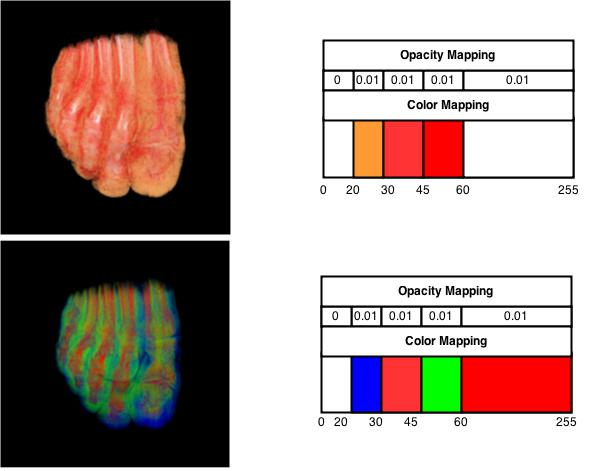
\includegraphics[width=350pt]{Images/foot_different_TF.jpg}
\caption{\label{fig:ray_cast1.jpg} Application of two different 1D transfer
functions on the same dataset. The transfer functions are shown next to their corresponding image.}
\end{figure} 


\subsection{Region of Interest}
A region of interest (often abbreviated ROI), is a selected subset of samples within a dataset identified for a particular purpose. A ROI can be any of the following.

\begin{itemize}
\item Volume of Interest, which is specified as a range of voxels within an 3D volume. For example, we could define a cubic, spherical or cylindrical ROI. 
\item A range of voxel intensities can also be a ROI.
\item A range of voxel intensities of one modality can be defined as an ROI in a multi-modal setup. 
\end{itemize}

\section{Volume Ray Casting}

Raycasting is a technique to visualize volume data. It is method in which for every pixel in the image, a ray is cast through the volume parallel to the view direction. The ray intersects(or passes close to) a line of voxels. The color of the pixel is computed based on color and transparency of the voxels that are intersected by the ray.

The ray equation is defined by a starting point and a direction, as shown in figure 2.2. If the ray hits the volume, the color of the pixel is calculated by sampling the data values of the ray at a finite number of positions in the volume. On each sample the transfer function is applied and composited with accumulated values of the ray.

\begin{figure}
\centering
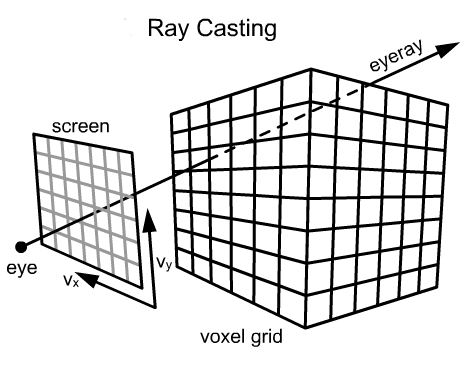
\includegraphics[width=220pt]{Images/ray_cast1.jpg}
\caption{\label{fig:ray_cast1.jpg} Direct volume rendering using raycasting.}
\end{figure}


\subsection{Basic Algorithm}

In its basic form, the volume ray casting algorithm comprises of a ray being cast through the volume, for each pixel of the final image. Generally, the volume is enclosed within a bounding primitive, a simple geometric object -- usually a cuboid -- that is used to intersect the ray of sight and the volume. Along the part of the ray of sight that lies within the volume, equidistant sampling points or samples are selected. In general, the volume is not aligned with the ray of sight, and sampling points will usually be located in between voxels. Because of that, it is necessary to interpolate the values of the samples from its surrounding voxels. After all sampling points have been fetched, they are composited along the ray of sight, resulting in the final color value for the pixel that is currently being processed. This compositing technique is explained in detail in a later section.

\subsection{Two-pass Rendering}

To perform raycasting on  a volume for an arbitrary view direction, we need to compute the points at which each ray enters and exits the cube corresponding to  the volume. An efficient and convenient method for this is to render the front and back faces of the cube into separate images, as shown in figure 2.4. The same pixel coordinates on the two images correspond to the images of points on a given ray, and specifically the entry and exit points of the ray. Thus, by tracking the mapping from points on the cube faces to the pixels on the images, we can compute the entry and exit point for each ray. \\



\begin{figure}
\centering
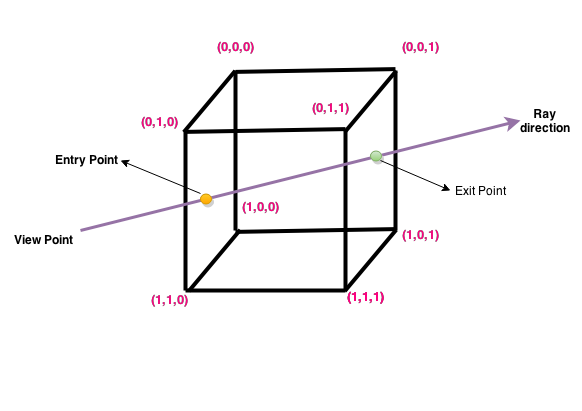
\includegraphics[width=320pt]{Images/cube.png}
\caption{\label{fig:ray_cast1.jpg} Assigning unique colors to all corners to the bounding box.}
\end{figure}


\lstdefinestyle{customc}{
  belowcaptionskip=1\baselineskip,
  breaklines=true,
  frame=L,
  xleftmargin=\parindent,
  language=C,
  showstringspaces=false,
  basicstyle=\footnotesize\ttfamily,
  keywordstyle=\bfseries\color{green!40!black},
  commentstyle=\itshape\color{purple!40!black},
  identifierstyle=\color{blue},
  stringstyle=\color{orange},
}


\lstset{style=customc}

\textbf{Pseudocode of Two-pass Volume ray casting:} 
\\
\begin{lstlisting}
First pass: render the backface of the boundbox  
Second pass: render the frontface of the boundbox
Lookup volume exit position from backface 2D texture 
Entry position obtained at second pass    
Compute ray of sight direction  

While in volume  
        Lookup data value at ray position  
        Apply transfer function to data value  
        Accumulate color and opacity  
        Advance along ray  
\end{lstlisting}	

We use two float-textures, where the color value encodes the co-ordinates of the entry and respectively the exit points. To obtain intersection of the ray of sight with data volume, we use a bounding box, which is a cube with each edge of unit length. Each of the eight corner vertex of the cube are assigned unique colors, as shown in figure 2.3. During rendering,  OpenGL will interpolate the color values between the vertices automatically. Since the corner colors are unique, we can use the interpolated colour values of a pixel to reconstruct the 3D coordinates of the intersection points of the ray of sight. On finding the entry and exit points on the cube, ray direction is easily obtained. From the entry point, ray starts marching towards the exit point while sampling points at equidistant locations.

\begin{figure}[!h]
\centering
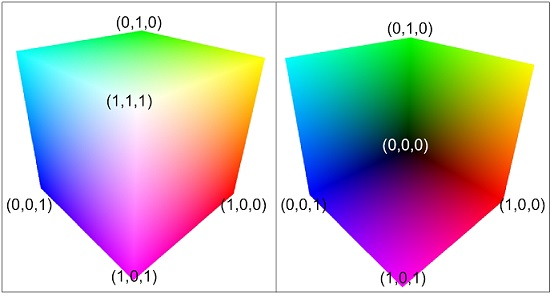
\includegraphics[width=350pt]{Images/ray_entry_exit.jpg}
\caption{\label{fig:ray_cast1.jpg} Entry and exit Textures.}
\end{figure}


\subsection{Sampling} 

Along the part of the ray of sight that lies within the volume, equidistant sampling points or samples are selected. In general, the volume is not aligned with the ray of sight, and sampling points will usually be located in between voxels, as shown in figure 2.5. Because of that, it is necessary to interpolate the values of the samples from its surrounding voxels. 

\begin{figure}[h]
\centering
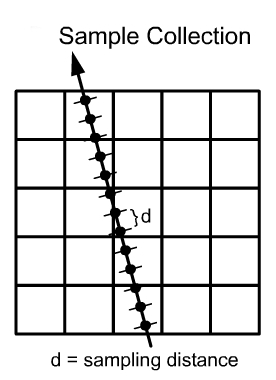
\includegraphics[width=120pt]{Images/sampling1.jpg}
\caption{\label{fig:ray_cast1.jpg} Sampling along the direction of ray.}
\end{figure}

\subsection{Compositing }

The discrete version of the volume rendering equation replaces the continuous integral with a Riemann sum. 

Discrete Volume Rendering Equations:

\begin{equation}
 C \; = \; \sum\limits_{i-1}^{n} \; C_i \; \prod\limits_{j=1}^{i-1} \; ( 1 \; - \; A_j) 
\end{equation}         
\begin{equation}
 A \; = 1 \; - \; \prod\limits_{j=1}^{n} \; ( 1 \; - \; A_j) 
\end{equation}

Here, Opacity $A_i$ approximates the absorption and opacity-weighted color $C_i$ approximates the emission and the absorption along the ray segment between samples i and i+1. 

This formula is efficiently evaluated by sorting the samples along the viewing ray and computing the accumulated color C and opacity A iteratively. The color of each sample is determined by classification and shading, and when the transparency is determined by classification, the next step is to evaluate the volume rendering equation using these values. This evaluation is performed by a process called compositing which generates the final pixel value for a ray shot into the volume. Two techniques for compositing  are front-to-back and back-to-front compositing.


\subsubsection{Back-to-Front Compositing Equations}

In this technique, samples are sorted in back-to-front order, and the accumulated color and opacity are computed iteratively. A single step of the compositing process is known as the Over Operator. 
 
\begin{equation}
\hat{C}_i \; = \; C_i \; + \; (1 \; - \; A_i ) \; \hat{C}_{i+1} 
\end{equation}
\begin{equation}
\hat{A}_i \; = \; A_i \; + \; (1 \; - \; A_i ) \; \hat{A}_{i+1} 
\end{equation}

where, ${C}_i$ and ${A}_i$ are the color and opacity obtained from the fragment shading stage for the ray i, along the viewing direction, and $\hat{C}_i$ is the accumulated color from the back of the volume.

\subsubsection{Front-to-Back Compositiong Equations}
In this technique, samples are sorted in front-to-back order. Front-to-back compositing has an added advantage over back-to-front compositing. Since the composition is done towards the back and the current transparency is known at all times, the compositing can be stopped early when the opacity is above a threshold (since nothing behind that point is going to affect the final image). This is one of the more powerful optimizations that can be done for several rendering techniques. \\

The front to back equation is:
\begin{equation}
\hat{C}_i \; = \; (1 \; - \; \hat{A}_{i-1} \; ) \; C_i \; + \; \hat{C}_{i-1}    
\end{equation}
\begin{equation}
\hat{A}_i \; = \; (1 \; - \; \hat{A}_{i-1} \; ) \; A_i \; + \; \hat{A}_{i-1}    
\end{equation}

where $\hat{C}_i \; and \; \hat{A}_i$ are the accumulated color and opacity from the front of the volume. 


\begin{figure}[h]
\centering
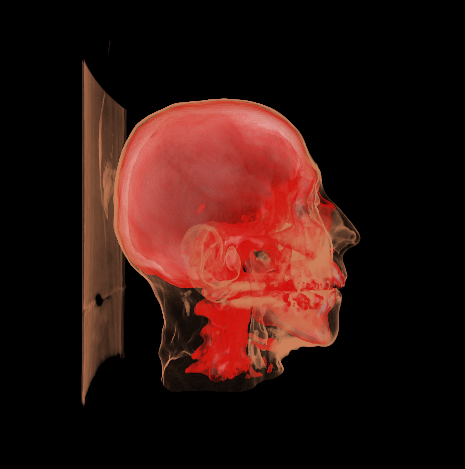
\includegraphics[width=220pt]{Images/dvr_head.png}
\caption{\label{fig:ray_cast1.jpg} Direct volume rendering of a volumetric head dataset.}
\end{figure}


